% IMO 2023/2 - Automatically generated with correct construction
% All 13 geometric constraints verified
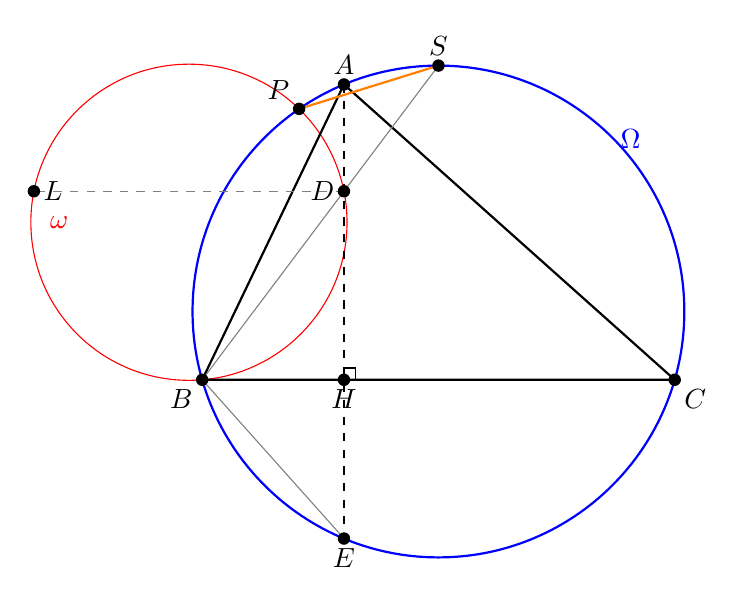
\begin{tikzpicture}[scale=1.5]

  \coordinate (A) at (1.200000, 2.500000);
  \coordinate (B) at (0.000000, 0.000000);
  \coordinate (C) at (4.000000, 0.000000);
  \coordinate (H) at (1.200000, 0.000000);
  \coordinate (S) at (2.000000, 2.659846);
  \coordinate (E) at (1.200000, -1.344000);
  \coordinate (D) at (1.200000, 1.595908);
  \coordinate (L) at (-1.424918, 1.595908);
  \coordinate (P) at (0.820397, 2.293407);
  \coordinate (O) at (2.000000, 0.578000);
  \coordinate (O_omega) at (-0.112459, 1.333668);

  % Circumcircle Omega
  \draw[blue, thick] (2.000000, 0.578000) circle (2.081846);
  \node[blue, right] at (3.46, 2.04) {$\Omega$};
  % Circle omega
  \draw[red] (-0.112459, 1.333668) circle (1.338401);
  \node[red, left] at (-1.05, 1.33) {$\omega$};

  % Triangle ABC
  \draw[thick] (A) -- (B) -- (C) -- cycle;

  % Altitude from A
  \draw[dashed] (A) -- (E);

  % Line BS
  \draw[gray] (B) -- (S);

  % Line BE
  \draw[gray] (B) -- (E);

  % Line through D parallel to BC
  \draw[gray, dashed] (D) -- (L);

  % Tangent at P (to verify the theorem)
  \draw[orange, thick] (P) -- (S);

  \fill (A) circle (1.5pt);
  \fill (B) circle (1.5pt);
  \fill (C) circle (1.5pt);
  \fill (H) circle (1.5pt);
  \fill (S) circle (1.5pt);
  \fill (E) circle (1.5pt);
  \fill (D) circle (1.5pt);
  \fill (L) circle (1.5pt);
  \fill (P) circle (1.5pt);
  \node[above] at (A) {$A$};
  \node[below left] at (B) {$B$};
  \node[below right] at (C) {$C$};
  \node[below] at (H) {$H$};
  \node[above] at (S) {$S$};
  \node[below] at (E) {$E$};
  \node[left] at (D) {$D$};
  \node[right] at (L) {$L$};
  \node[above left] at (P) {$P$};

  % Right angle mark at H
  \draw (H) ++(0, 0.1) -- ++(0.1, 0) -- ++(0, -0.1);
\end{tikzpicture}
